%This is chapter 1
%%=========================================
%% Defining listings.
\lstset{
emph={def,for,each,in,if,elif,else,while,return,True,False,bool,do}, 
emphstyle={\textbf}, 
captionpos=b,
literate=%
  {Ö}{{\"O}}1
  {Ä}{{\"A}}1
  {Ü}{{\"U}}1
  {ß}{{\ss}}1
  {ü}{{\"u}}1
  {ä}{{\"a}}1
  {ö}{{\"o}}1
}
%%=========================================
\begingroup
\renewcommand{\cleardoublepage}{}
\renewcommand{\clearpage}{}
\chapter{Introduction}
\endgroup
\iffalse
We say a text \textit{T} entails a second text, \textit{H}, also known as \textit{hypothesis}, if a human reading both T and H would infer that the meaning of H follows from the meaning of T. \cite{dagan2006pascal}\\
Textual Entailment plays a role in many systems, such as Question Answering \cite{ferrandez2008improving}, Machine Translation \cite{pado2009textual} or Text Summarization \cite{gupta2014text} tasks. One sub field of Textual Entailment tasks is \textit{Knowledge Extraction and Representation} for use in Textual Entailment systems.\\
\fi
One approach to find or reject textual entailment between two texts is to use world knowledge infer the entailment. World knowledge refers to specific knowledge such as \textit{An apple is a fruit.} or \textit{Fire is hot}. Using this information it becomes possible to infer entailment between the text pairs.
\begin{minipage}{0.6\textwidth}
\begin{figure}[H]
    \centering
    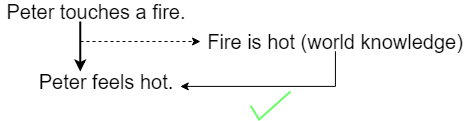
\includegraphics[scale=0.53]{fig/world_knowledge}
    \caption{Example usage of world knowledge to infer textual entailment}
    \label{fig:world-knowledge}
\end{figure}
\end{minipage}
\begin{minipage}{0.4\textwidth}
To have this sort of knowledge available for use in a textual entailment system it is necessary to extract it and then represent the knowledge in some way.\\
\end{minipage}
An example of such a work is \cite{silva2018recognizing}. The work makes use of WordNet \cite{miller1995wordnet} to create a \textit{knowledge graph} over the definitions contained therein. A graph navigational algorithm is then used to find paths between pairs of nodes, where the nodes represent knowledge extracted from the WordNet definitions, to find textual entailment between pairs of texts and use the path taken in the knowledge to create a human readable justification of why there is an entailment, if an entailment is found.\\
The knowledge found in WordNet however is limited. The definitions are rather short and do not contain instance specific knowledge. The definition for \textit{cellphone} from WordNet is as follows:
\begin{quote}
a hand-held mobile radiotelephone for use in an area divided into small sections, each with its own short-range transmitter/receive
\end{quote}
This definition does not include that modern phones have built-in cameras or the capability to run apps, among other things. Even if such information was included, it does not help when working with specific instances of a type, such as a \textit{specific} cellphone.\\
To alleviate this problem I have built a system that extracts instance specific, qualitative world knowledge from product reviews over specific products based on \cite{scaffidi2007red} and have added the extracted information into the knowledge graph used in \cite{silva2018recognizing} to answer simple queries over specific product instances.\\
The category of products that is used to showcase the system is \textit{cellphones}. The goal of this seminar topic is not to build a full-fledged system but rather show how the definitional knowledge graph can be extended with information extracted from product reviews and how this knowledge can be used in a textual entailment context, by showcasing a very basic Question Answering system.